\documentclass[border=4pt]{standalone}
\usepackage{amsmath,amssymb}
\usepackage{pgfplots}
\pgfplotsset{compat=1.17}
\usetikzlibrary{arrows.meta,positioning,calc}
\begin{document}
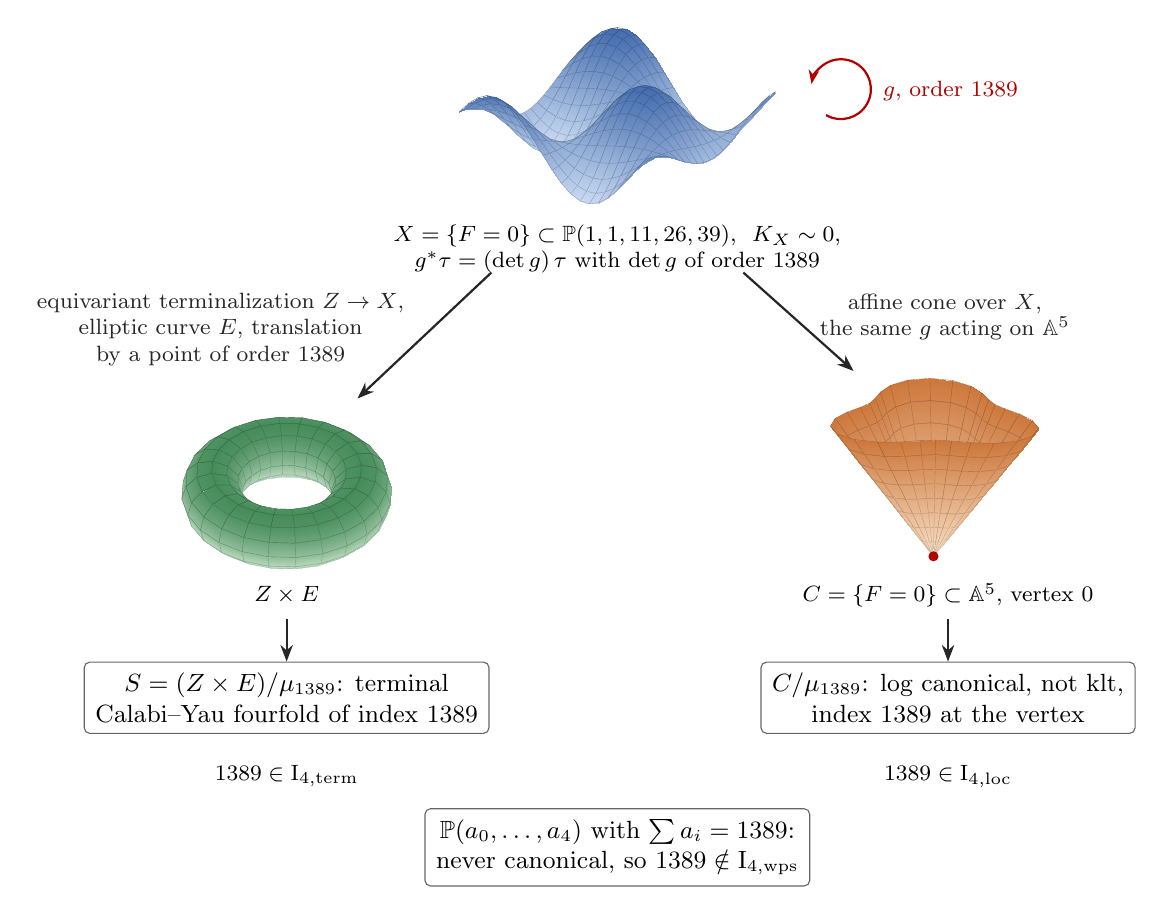
\begin{tikzpicture}[
  arrowstep/.style={-{Stealth[length=6pt]},line width=0.8pt,gray!30!black},
  lab/.style={font=\footnotesize,align=center},
  res/.style={font=\small,align=center,draw=black!60,rounded corners=2pt,inner sep=4pt,fill=white}]
% ---------- the threefold X with its symmetry ----------
\begin{axis}[at={(4.6cm,5.0cm)},anchor=center,width=5.6cm,height=4.4cm,hide axis,
  view={35}{38},colormap={b}{rgb255=(205,222,245) rgb255=(70,110,175)},z buffer=sort]
  \addplot3[surf,shader=faceted interp,draw=black!35,line width=0.15pt,samples=21,domain=-180:180,y domain=-180:180]
    ({x/60},{y/60},{0.55*sin(x)*cos(y)+0.25*cos(x+y)});
\end{axis}
\draw[-{Stealth[length=5pt]},line width=0.8pt,red!70!black] (7.25,5.05) arc[start angle=-120,end angle=170,radius=0.38];
\node[lab,red!70!black,anchor=west] at (7.85,5.35) {$g$, order $1389$};
\node[lab] at (4.6,3.35) {$X=\{F=0\}\subset\mathbb P(1,1,11,26,39)$, \ $K_X\sim0$,\\ $g^*\tau=(\det g)\,\tau$ with $\det g$ of order $1389$};
% ---------- left: the fourfold ----------
\begin{axis}[at={(0.4cm,0.25cm)},anchor=center,width=5.4cm,height=4.6cm,hide axis,
  view={25}{38},colormap={g}{rgb255=(220,240,220) rgb255=(70,140,90)},z buffer=sort,
  unit vector ratio=1 1 1,scale only axis=false]
  \addplot3[surf,shader=faceted interp,draw=black!30,line width=0.15pt,samples=25,samples y=13,domain=0:360,y domain=0:360]
    ({(2+0.8*cos(y))*cos(x)},{(2+0.8*cos(y))*sin(x)},{0.8*sin(y)});
\end{axis}
\node[lab] at (0.4,-1.05) {$Z\times E$};
\draw[arrowstep] (3.0,3.05) -- node[lab,left=6pt,pos=0.45]{equivariant terminalization $Z\to X$,\\ elliptic curve $E$, translation\\ by a point of order $1389$} (1.3,1.45);
% ---------- right: the cone ----------
\begin{axis}[at={(8.8cm,0.3cm)},anchor=center,width=5.0cm,height=4.9cm,hide axis,
  view={30}{22},colormap={o}{rgb255=(250,226,200) rgb255=(205,120,60)},z buffer=sort]
  \addplot3[surf,shader=faceted interp,draw=black!30,line width=0.15pt,samples=31,samples y=9,domain=0:360,y domain=0:1]
    ({y*cos(x)*(1+0.22*cos(3*x))},{y*sin(x)*(1+0.22*cos(3*x))},{y});
  \addplot3[only marks,mark=*,mark size=1.6pt,red!70!black] coordinates {(0,0,0)};
\end{axis}
\node[lab] at (8.8,-1.05) {$C=\{F=0\}\subset\mathbb A^5$, vertex $0$};
\draw[arrowstep] (6.2,3.05) -- node[lab,right=6pt,pos=0.45]{affine cone over $X$,\\ the same $g$ acting on $\mathbb A^5$} (7.6,1.8);
% ---------- results ----------
\node[res] (S) at (0.4,-2.35) {$S=(Z\times E)/\mu_{1389}$: terminal\\ Calabi--Yau fourfold of index $1389$};
\node[res] (Y) at (8.8,-2.35) {$C/\mu_{1389}$: log canonical, not klt,\\ index $1389$ at the vertex};
\node[res] (W) at (4.6,-4.25) {$\mathbb P(a_0,\dots,a_4)$ with $\sum a_i=1389$:\\ never canonical, so $1389\notin\mathrm I_{4,\mathrm{wps}}$};
\draw[arrowstep] (0.4,-1.35)--(S.north);
\draw[arrowstep] (8.8,-1.35)--(Y.north);
\node[lab] at (0.4,-3.35) {$1389\in\mathrm I_{4,\mathrm{term}}$};
\node[lab] at (8.8,-3.35) {$1389\in\mathrm I_{4,\mathrm{loc}}$};
\end{tikzpicture}
\end{document}
